\documentclass[twoside]{book}

% Packages required by doxygen
\usepackage{fixltx2e}
\usepackage{calc}
\usepackage{doxygen}
\usepackage[export]{adjustbox} % also loads graphicx
\usepackage{graphicx}
\usepackage[utf8]{inputenc}
\usepackage{makeidx}
\usepackage{multicol}
\usepackage{multirow}
\PassOptionsToPackage{warn}{textcomp}
\usepackage{textcomp}
\usepackage[nointegrals]{wasysym}
\usepackage[table]{xcolor}

% Font selection
\usepackage[T1]{fontenc}
\usepackage[scaled=.90]{helvet}
\usepackage{courier}
\usepackage{amssymb}
\usepackage{sectsty}
\renewcommand{\familydefault}{\sfdefault}
\allsectionsfont{%
  \fontseries{bc}\selectfont%
  \color{darkgray}%
}
\renewcommand{\DoxyLabelFont}{%
  \fontseries{bc}\selectfont%
  \color{darkgray}%
}
\newcommand{\+}{\discretionary{\mbox{\scriptsize$\hookleftarrow$}}{}{}}

% Page & text layout
\usepackage{geometry}
\geometry{%
  a4paper,%
  top=2.5cm,%
  bottom=2.5cm,%
  left=2.5cm,%
  right=2.5cm%
}
\tolerance=750
\hfuzz=15pt
\hbadness=750
\setlength{\emergencystretch}{15pt}
\setlength{\parindent}{0cm}
\setlength{\parskip}{0.2cm}
\makeatletter
\renewcommand{\paragraph}{%
  \@startsection{paragraph}{4}{0ex}{-1.0ex}{1.0ex}{%
    \normalfont\normalsize\bfseries\SS@parafont%
  }%
}
\renewcommand{\subparagraph}{%
  \@startsection{subparagraph}{5}{0ex}{-1.0ex}{1.0ex}{%
    \normalfont\normalsize\bfseries\SS@subparafont%
  }%
}
\makeatother

% Headers & footers
\usepackage{fancyhdr}
\pagestyle{fancyplain}
\fancyhead[LE]{\fancyplain{}{\bfseries\thepage}}
\fancyhead[CE]{\fancyplain{}{}}
\fancyhead[RE]{\fancyplain{}{\bfseries\leftmark}}
\fancyhead[LO]{\fancyplain{}{\bfseries\rightmark}}
\fancyhead[CO]{\fancyplain{}{}}
\fancyhead[RO]{\fancyplain{}{\bfseries\thepage}}
\fancyfoot[LE]{\fancyplain{}{}}
\fancyfoot[CE]{\fancyplain{}{}}
\fancyfoot[RE]{\fancyplain{}{\bfseries\scriptsize Generated on Mon Apr 13 2015 18\+:21\+:31 for Top\+Down\+R\+P\+G by Doxygen }}
\fancyfoot[LO]{\fancyplain{}{\bfseries\scriptsize Generated on Mon Apr 13 2015 18\+:21\+:31 for Top\+Down\+R\+P\+G by Doxygen }}
\fancyfoot[CO]{\fancyplain{}{}}
\fancyfoot[RO]{\fancyplain{}{}}
\renewcommand{\footrulewidth}{0.4pt}
\renewcommand{\chaptermark}[1]{%
  \markboth{#1}{}%
}
\renewcommand{\sectionmark}[1]{%
  \markright{\thesection\ #1}%
}

% Indices & bibliography
\usepackage{natbib}
\usepackage[titles]{tocloft}
\setcounter{tocdepth}{3}
\setcounter{secnumdepth}{5}
\makeindex

% Hyperlinks (required, but should be loaded last)
\usepackage{ifpdf}
\ifpdf
  \usepackage[pdftex,pagebackref=true]{hyperref}
\else
  \usepackage[ps2pdf,pagebackref=true]{hyperref}
\fi
\hypersetup{%
  colorlinks=true,%
  linkcolor=blue,%
  citecolor=blue,%
  unicode%
}

% Custom commands
\newcommand{\clearemptydoublepage}{%
  \newpage{\pagestyle{empty}\cleardoublepage}%
}


%===== C O N T E N T S =====

\begin{document}

% Titlepage & ToC
\hypersetup{pageanchor=false,
             bookmarks=true,
             bookmarksnumbered=true,
             pdfencoding=unicode
            }
\pagenumbering{roman}
\begin{titlepage}
\vspace*{7cm}
\begin{center}%
{\Large Top\+Down\+R\+P\+G }\\
\vspace*{1cm}
{\large Generated by Doxygen 1.8.9.1}\\
\vspace*{0.5cm}
{\small Mon Apr 13 2015 18:21:31}\\
\end{center}
\end{titlepage}
\clearemptydoublepage
\tableofcontents
\clearemptydoublepage
\pagenumbering{arabic}
\hypersetup{pageanchor=true}

%--- Begin generated contents ---
\chapter{Hierarchical Index}
\section{Class Hierarchy}
This inheritance list is sorted roughly, but not completely, alphabetically\+:\begin{DoxyCompactList}
\item \contentsline{section}{R\+P\+G\+Object.\+Attribut\+Modification\+Helper}{\pageref{class_r_p_g_object_1_1_attribut_modification_helper}}{}
\item \contentsline{section}{Content}{\pageref{struct_content}}{}
\item \contentsline{section}{Effect\+Script\+Object}{\pageref{class_effect_script_object}}{}
\item \contentsline{section}{T\+Creature.\+Equipment\+Slot}{\pageref{struct_t_creature_1_1_equipment_slot}}{}
\item \contentsline{section}{R\+P\+G\+Object.\+Attribut\+Modification\+Helper.\+Inhibitor}{\pageref{class_r_p_g_object_1_1_attribut_modification_helper_1_1_inhibitor}}{}
\item \contentsline{section}{I\+R\+P\+G\+Source}{\pageref{interface_i_r_p_g_source}}{}
\begin{DoxyCompactList}
\item \contentsline{section}{R\+P\+G\+Object}{\pageref{class_r_p_g_object}}{}
\begin{DoxyCompactList}
\item \contentsline{section}{Interactive\+Object}{\pageref{class_interactive_object}}{}
\item \contentsline{section}{T\+Creature}{\pageref{class_t_creature}}{}
\item \contentsline{section}{T\+Item}{\pageref{class_t_item}}{}
\begin{DoxyCompactList}
\item \contentsline{section}{T\+Equipment}{\pageref{class_t_equipment}}{}
\end{DoxyCompactList}
\end{DoxyCompactList}
\item \contentsline{section}{T\+Effect}{\pageref{class_t_effect}}{}
\end{DoxyCompactList}
\item \contentsline{section}{R\+P\+G\+Object.\+Attribut\+Modification\+Helper.\+Modification}{\pageref{class_r_p_g_object_1_1_attribut_modification_helper_1_1_modification}}{}
\item Mono\+Behaviour\begin{DoxyCompactList}
\item \contentsline{section}{Core}{\pageref{class_core}}{}
\item \contentsline{section}{R\+P\+G\+Object}{\pageref{class_r_p_g_object}}{}
\end{DoxyCompactList}
\item \contentsline{section}{Effect\+Script\+Object.\+Numeric\+Value}{\pageref{class_effect_script_object_1_1_numeric_value}}{}
\item \contentsline{section}{Effect\+Script\+Object.\+Paramter}{\pageref{struct_effect_script_object_1_1_paramter}}{}
\item \contentsline{section}{Effect\+Script\+Object.\+String\+Value}{\pageref{class_effect_script_object_1_1_string_value}}{}
\item \contentsline{section}{T\+Item\+Statistic}{\pageref{class_t_item_statistic}}{}
\item \contentsline{section}{R\+P\+G\+Object.\+Value\+Helper}{\pageref{class_r_p_g_object_1_1_value_helper}}{}
\begin{DoxyCompactList}
\item \contentsline{section}{R\+P\+G\+Object.\+boolean\+Value\+Helper}{\pageref{class_r_p_g_object_1_1boolean_value_helper}}{}
\item \contentsline{section}{R\+P\+G\+Object.\+Numeric\+Value\+Helper}{\pageref{class_r_p_g_object_1_1_numeric_value_helper}}{}
\end{DoxyCompactList}
\end{DoxyCompactList}

\chapter{Class Index}
\section{Class List}
Here are the classes, structs, unions and interfaces with brief descriptions\+:\begin{DoxyCompactList}
\item\contentsline{section}{\hyperlink{class_r_p_g_object_1_1_attribut_modification_helper}{R\+P\+G\+Object.\+Attribut\+Modification\+Helper} \\*Diese Klasse verwaltet die Modifikationen für den genannten Wert, die sich aus den passiven Teilen aller Effekte ergeben }{\pageref{class_r_p_g_object_1_1_attribut_modification_helper}}{}
\item\contentsline{section}{\hyperlink{class_r_p_g_object_1_1boolean_value_helper}{R\+P\+G\+Object.\+boolean\+Value\+Helper} }{\pageref{class_r_p_g_object_1_1boolean_value_helper}}{}
\item\contentsline{section}{\hyperlink{struct_content}{Content} }{\pageref{struct_content}}{}
\item\contentsline{section}{\hyperlink{class_core}{Core} }{\pageref{class_core}}{}
\item\contentsline{section}{\hyperlink{class_effect_script_object}{Effect\+Script\+Object} }{\pageref{class_effect_script_object}}{}
\item\contentsline{section}{\hyperlink{struct_t_creature_1_1_equipment_slot}{T\+Creature.\+Equipment\+Slot} }{\pageref{struct_t_creature_1_1_equipment_slot}}{}
\item\contentsline{section}{\hyperlink{class_r_p_g_object_1_1_attribut_modification_helper_1_1_inhibitor}{R\+P\+G\+Object.\+Attribut\+Modification\+Helper.\+Inhibitor} }{\pageref{class_r_p_g_object_1_1_attribut_modification_helper_1_1_inhibitor}}{}
\item\contentsline{section}{\hyperlink{class_interactive_object}{Interactive\+Object} }{\pageref{class_interactive_object}}{}
\item\contentsline{section}{\hyperlink{interface_i_r_p_g_source}{I\+R\+P\+G\+Source} }{\pageref{interface_i_r_p_g_source}}{}
\item\contentsline{section}{\hyperlink{class_r_p_g_object_1_1_attribut_modification_helper_1_1_modification}{R\+P\+G\+Object.\+Attribut\+Modification\+Helper.\+Modification} }{\pageref{class_r_p_g_object_1_1_attribut_modification_helper_1_1_modification}}{}
\item\contentsline{section}{\hyperlink{class_effect_script_object_1_1_numeric_value}{Effect\+Script\+Object.\+Numeric\+Value} }{\pageref{class_effect_script_object_1_1_numeric_value}}{}
\item\contentsline{section}{\hyperlink{class_r_p_g_object_1_1_numeric_value_helper}{R\+P\+G\+Object.\+Numeric\+Value\+Helper} }{\pageref{class_r_p_g_object_1_1_numeric_value_helper}}{}
\item\contentsline{section}{\hyperlink{struct_effect_script_object_1_1_paramter}{Effect\+Script\+Object.\+Paramter} }{\pageref{struct_effect_script_object_1_1_paramter}}{}
\item\contentsline{section}{\hyperlink{class_r_p_g_object}{R\+P\+G\+Object} \\*Diese Basisklasse vereinheitlicht die wichtigsten Eigenschaften aller Objekte, die Teil der vom R\+P\+G-\/\+System verwalteten Welt sind }{\pageref{class_r_p_g_object}}{}
\item\contentsline{section}{\hyperlink{class_t_creature_1_1_skill}{T\+Creature.\+Skill} \\*Klasse zum bereitstellen von Talentinformationen }{\pageref{class_t_creature_1_1_skill}}{}
\item\contentsline{section}{\hyperlink{class_effect_script_object_1_1_string_value}{Effect\+Script\+Object.\+String\+Value} }{\pageref{class_effect_script_object_1_1_string_value}}{}
\item\contentsline{section}{\hyperlink{class_t_creature}{T\+Creature} }{\pageref{class_t_creature}}{}
\item\contentsline{section}{\hyperlink{struct_t_discipline___template}{T\+Discipline\+\_\+\+Template} \\*Diese Struktur dient der Verwaltung aller Vorlagen für Disziplinen, aus ihr wird das Rohgerüst in der Creature generiert und später erweitert }{\pageref{struct_t_discipline___template}}{}
\item\contentsline{section}{\hyperlink{class_t_effect}{T\+Effect} }{\pageref{class_t_effect}}{}
\item\contentsline{section}{\hyperlink{class_t_equipment}{T\+Equipment} }{\pageref{class_t_equipment}}{}
\item\contentsline{section}{\hyperlink{class_t_item}{T\+Item} }{\pageref{class_t_item}}{}
\item\contentsline{section}{\hyperlink{class_t_item_statistic}{T\+Item\+Statistic} }{\pageref{class_t_item_statistic}}{}
\item\contentsline{section}{\hyperlink{class_r_p_g_object_1_1_value_helper}{R\+P\+G\+Object.\+Value\+Helper} }{\pageref{class_r_p_g_object_1_1_value_helper}}{}
\end{DoxyCompactList}

\chapter{Class Documentation}
\hypertarget{class_r_p_g_object_1_1_attribut_modification_helper}{}\section{R\+P\+G\+Object.\+Attribut\+Modification\+Helper Class Reference}
\label{class_r_p_g_object_1_1_attribut_modification_helper}\index{R\+P\+G\+Object.\+Attribut\+Modification\+Helper@{R\+P\+G\+Object.\+Attribut\+Modification\+Helper}}
\subsection*{Classes}
\begin{DoxyCompactItemize}
\item 
class \hyperlink{class_r_p_g_object_1_1_attribut_modification_helper_1_1_inhibitor}{Inhibitor}
\item 
class \hyperlink{class_r_p_g_object_1_1_attribut_modification_helper_1_1_modification}{Modification}
\end{DoxyCompactItemize}
\subsection*{Public Member Functions}
\begin{DoxyCompactItemize}
\item 
\hypertarget{class_r_p_g_object_1_1_attribut_modification_helper_a77b155c4033c277b394c6d6fa9017788}{}{\bfseries Attribut\+Modification\+Helper} (string Name)\label{class_r_p_g_object_1_1_attribut_modification_helper_a77b155c4033c277b394c6d6fa9017788}

\end{DoxyCompactItemize}
\subsection*{Public Attributes}
\begin{DoxyCompactItemize}
\item 
\hypertarget{class_r_p_g_object_1_1_attribut_modification_helper_a7d284a483e95ba8c7de9f536f50fd395}{}string {\bfseries Attribute\+Name}\label{class_r_p_g_object_1_1_attribut_modification_helper_a7d284a483e95ba8c7de9f536f50fd395}

\item 
\hypertarget{class_r_p_g_object_1_1_attribut_modification_helper_a16d781421788573ab938f850f57bda0a}{}List$<$ List$<$ \hyperlink{class_r_p_g_object_1_1_attribut_modification_helper_1_1_modification}{Modification} $>$ $>$ {\bfseries All\+Modifications} = new List$<$List$<$\hyperlink{class_r_p_g_object_1_1_attribut_modification_helper_1_1_modification}{Modification}$>$$>$ ()\label{class_r_p_g_object_1_1_attribut_modification_helper_a16d781421788573ab938f850f57bda0a}

\item 
\hypertarget{class_r_p_g_object_1_1_attribut_modification_helper_a6d8cb9272270fecb0d7aaf8df7ef184d}{}List$<$ \hyperlink{class_r_p_g_object_1_1_attribut_modification_helper_1_1_inhibitor}{Inhibitor} $>$ {\bfseries Inhibitors} = new List$<$\hyperlink{class_r_p_g_object_1_1_attribut_modification_helper_1_1_inhibitor}{Inhibitor}$>$ ()\label{class_r_p_g_object_1_1_attribut_modification_helper_a6d8cb9272270fecb0d7aaf8df7ef184d}

\end{DoxyCompactItemize}
\subsection*{Properties}
\begin{DoxyCompactItemize}
\item 
\hypertarget{class_r_p_g_object_1_1_attribut_modification_helper_a420f306ba1d89f6dbfa12f98f7a86a23}{}List$<$ \hyperlink{class_r_p_g_object_1_1_attribut_modification_helper_1_1_modification}{Modification} $>$ {\bfseries Used\+Modifications}\hspace{0.3cm}{\ttfamily  \mbox{[}get\mbox{]}}\label{class_r_p_g_object_1_1_attribut_modification_helper_a420f306ba1d89f6dbfa12f98f7a86a23}

\item 
\hypertarget{class_r_p_g_object_1_1_attribut_modification_helper_ad17e7c9081ae8e2e5c33dfa4bd114f9b}{}float {\bfseries Overall\+Modification}\hspace{0.3cm}{\ttfamily  \mbox{[}get\mbox{]}}\label{class_r_p_g_object_1_1_attribut_modification_helper_ad17e7c9081ae8e2e5c33dfa4bd114f9b}

\end{DoxyCompactItemize}


The documentation for this class was generated from the following file\+:\begin{DoxyCompactItemize}
\item 
C\+:/\+Users/\+Jordan Eichner/\+Documents/\+Unity/\+Top\+Down\+R\+P\+G/\+Assets/\+Standard\+Assets/\+R\+P\+G-\/\+Sources/\+Scripts/\+Meta/R\+P\+G\+Object.\+cs\end{DoxyCompactItemize}

\hypertarget{class_r_p_g_object_1_1boolean_value_helper}{}\section{R\+P\+G\+Object.\+boolean\+Value\+Helper Class Reference}
\label{class_r_p_g_object_1_1boolean_value_helper}\index{R\+P\+G\+Object.\+boolean\+Value\+Helper@{R\+P\+G\+Object.\+boolean\+Value\+Helper}}
Inheritance diagram for R\+P\+G\+Object.\+boolean\+Value\+Helper\+:\begin{figure}[H]
\begin{center}
\leavevmode
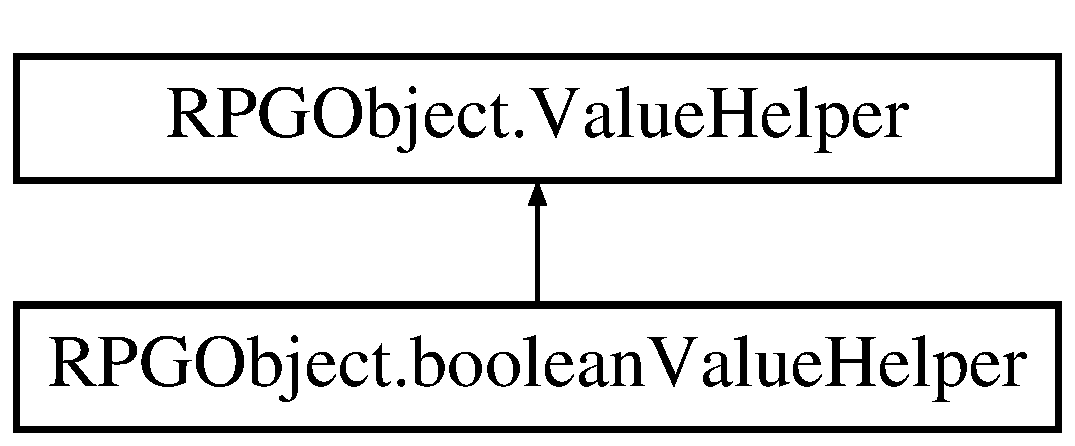
\includegraphics[height=2.000000cm]{class_r_p_g_object_1_1boolean_value_helper}
\end{center}
\end{figure}
\subsection*{Public Attributes}
\begin{DoxyCompactItemize}
\item 
\hypertarget{class_r_p_g_object_1_1boolean_value_helper_af964a85c583322a703930e4d6c0ba270}{}bool {\bfseries Value}\label{class_r_p_g_object_1_1boolean_value_helper_af964a85c583322a703930e4d6c0ba270}

\end{DoxyCompactItemize}


\subsection{Detailed Description}
Spezialisierte Hilfsklasse um boolsche Werte zu speichern 

The documentation for this class was generated from the following file\+:\begin{DoxyCompactItemize}
\item 
C\+:/\+Users/\+Jordan Eichner/\+Documents/\+Unity/\+Top\+Down\+R\+P\+G/\+Assets/\+Standard\+Assets/\+R\+P\+G-\/\+Sources/\+Scripts/\+Meta/R\+P\+G\+Object.\+cs\end{DoxyCompactItemize}

\hypertarget{struct_content}{}\section{Content Struct Reference}
\label{struct_content}\index{Content@{Content}}
\subsection*{Public Attributes}
\begin{DoxyCompactItemize}
\item 
\hypertarget{struct_content_a216f0b5c71894bbef26fc027895a8a39}{}string {\bfseries Information}\label{struct_content_a216f0b5c71894bbef26fc027895a8a39}

\item 
\hypertarget{struct_content_a8eee0e95f77c5d080aeab4a88cf5607d}{}string {\bfseries Strong\+Requirements}\label{struct_content_a8eee0e95f77c5d080aeab4a88cf5607d}

\item 
\hypertarget{struct_content_a8a0bbe78e06340e867bf694feddd4d1e}{}string {\bfseries Requirements}\label{struct_content_a8a0bbe78e06340e867bf694feddd4d1e}

\item 
\hypertarget{struct_content_a337b0374fcb40f66345cae16715e09d9}{}int {\bfseries Numberof\+Needed\+Requirments}\label{struct_content_a337b0374fcb40f66345cae16715e09d9}

\end{DoxyCompactItemize}


The documentation for this struct was generated from the following file\+:\begin{DoxyCompactItemize}
\item 
C\+:/\+Users/\+Jordan Eichner/\+Documents/\+Git\+Hub/\+Top\+Down\+R\+P\+G/\+Top\+Down\+R\+P\+G/\+Assets/\+Standard\+Assets/\+R\+P\+G libary/\+Scripts/\+Meta/Content.\+cs\end{DoxyCompactItemize}

\hypertarget{class_core}{}\section{Core Class Reference}
\label{class_core}\index{Core@{Core}}
Inheritance diagram for Core\+:\begin{figure}[H]
\begin{center}
\leavevmode
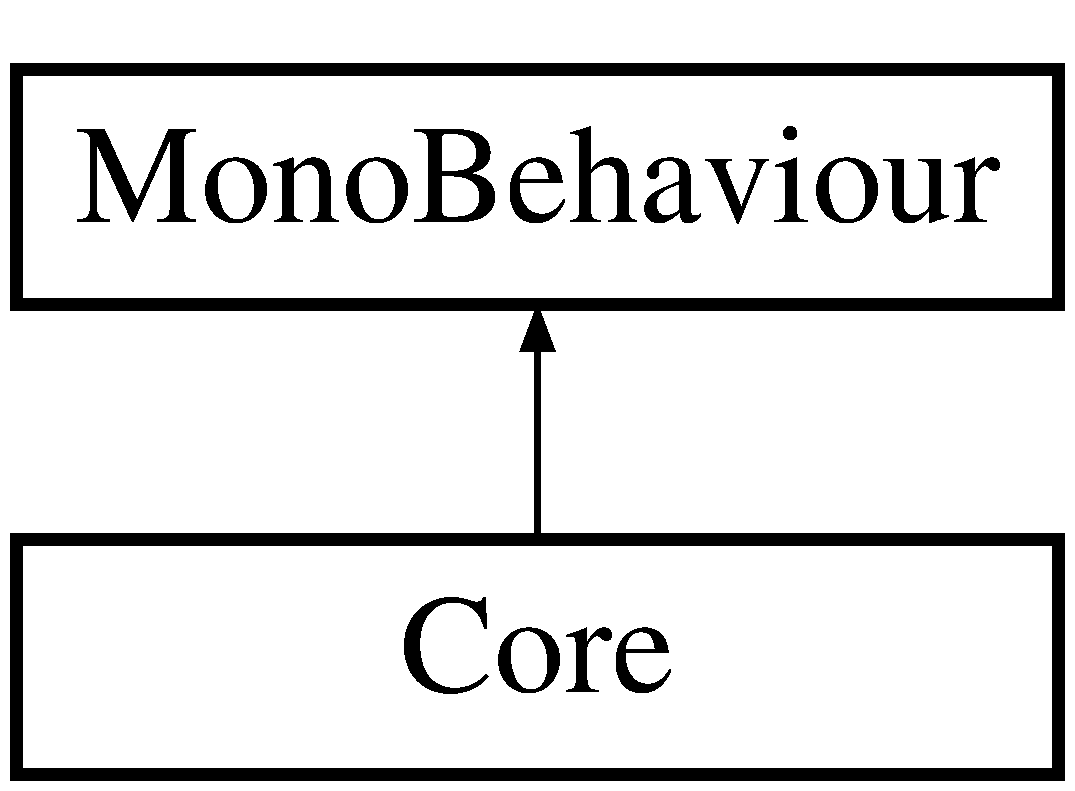
\includegraphics[height=2.000000cm]{class_core}
\end{center}
\end{figure}
\subsection*{Static Public Attributes}
\begin{DoxyCompactItemize}
\item 
\hypertarget{class_core_add8b471228af83cbf0723baefade84ea}{}static \hyperlink{class_core}{Core} {\bfseries instance}\label{class_core_add8b471228af83cbf0723baefade84ea}

\end{DoxyCompactItemize}


The documentation for this class was generated from the following file\+:\begin{DoxyCompactItemize}
\item 
C\+:/\+Users/\+Jordan Eichner/\+Documents/\+Git\+Hub/\+Top\+Down\+R\+P\+G/\+Top\+Down\+R\+P\+G/\+Assets/\+Standard\+Assets/\+R\+P\+G libary/\+Scripts/\+Meta/Core.\+cs\end{DoxyCompactItemize}

\hypertarget{class_effect_script_object}{}\section{Effect\+Script\+Object Class Reference}
\label{class_effect_script_object}\index{Effect\+Script\+Object@{Effect\+Script\+Object}}
\subsection*{Classes}
\begin{DoxyCompactItemize}
\item 
class \hyperlink{class_effect_script_object_1_1_numeric_value}{Numeric\+Value}
\item 
struct \hyperlink{struct_effect_script_object_1_1_paramter}{Paramter}
\item 
class \hyperlink{class_effect_script_object_1_1_string_value}{String\+Value}
\end{DoxyCompactItemize}
\subsection*{Public Member Functions}
\begin{DoxyCompactItemize}
\item 
\hypertarget{class_effect_script_object_ab6709e3186a3e37df774d961a06600a6}{}void {\bfseries On\+Activate} (\hyperlink{interface_i_r_p_g_source}{I\+R\+P\+G\+Source} s)\label{class_effect_script_object_ab6709e3186a3e37df774d961a06600a6}

\item 
\hypertarget{class_effect_script_object_a1f68ebfee4023bf30a52ea9408970523}{}{\bfseries Effect\+Script\+Object} (string \+\_\+\+Script, \hyperlink{interface_i_r_p_g_source}{I\+R\+P\+G\+Source} \+\_\+\+Source, \hyperlink{class_r_p_g_object}{R\+P\+G\+Object} \+\_\+\+Target, \hyperlink{class_t_effect}{T\+Effect} \+\_\+\+Effect)\label{class_effect_script_object_a1f68ebfee4023bf30a52ea9408970523}

\item 
\hypertarget{class_effect_script_object_aaa6b0f4677c9ee3de33693789ed271e4}{}void {\bfseries Set\+Up\+Effect} (\hyperlink{interface_i_r_p_g_source}{I\+R\+P\+G\+Source} \+\_\+\+Source, \hyperlink{class_r_p_g_object}{R\+P\+G\+Object} \+\_\+\+Target)\label{class_effect_script_object_aaa6b0f4677c9ee3de33693789ed271e4}

\end{DoxyCompactItemize}
\subsection*{Properties}
\begin{DoxyCompactItemize}
\item 
\hypertarget{class_effect_script_object_aa7393df152fc5f74e6e1090dee001506}{}bool {\bfseries Is\+Active}\hspace{0.3cm}{\ttfamily  \mbox{[}get\mbox{]}}\label{class_effect_script_object_aa7393df152fc5f74e6e1090dee001506}

\end{DoxyCompactItemize}


The documentation for this class was generated from the following file\+:\begin{DoxyCompactItemize}
\item 
C\+:/\+Users/\+Jordan Eichner/\+Documents/\+Unity/\+Top\+Down\+R\+P\+G/\+Assets/\+Standard\+Assets/\+R\+P\+G-\/\+Sources/\+Scripts/\+Effects/Effect\+Script\+Object.\+cs\end{DoxyCompactItemize}

\hypertarget{struct_t_creature_1_1_equipment_slot}{}\section{T\+Creature.\+Equipment\+Slot Struct Reference}
\label{struct_t_creature_1_1_equipment_slot}\index{T\+Creature.\+Equipment\+Slot@{T\+Creature.\+Equipment\+Slot}}
\subsection*{Public Attributes}
\begin{DoxyCompactItemize}
\item 
\hypertarget{struct_t_creature_1_1_equipment_slot_a4ce3ee475e08b0977d0fb59bfc60dc86}{}string {\bfseries Name}\label{struct_t_creature_1_1_equipment_slot_a4ce3ee475e08b0977d0fb59bfc60dc86}

\item 
\hypertarget{struct_t_creature_1_1_equipment_slot_aceb771e476871778c0518706dcdbe21d}{}\hyperlink{class_t_equipment}{T\+Equipment} {\bfseries Slotted\+Item}\label{struct_t_creature_1_1_equipment_slot_aceb771e476871778c0518706dcdbe21d}

\end{DoxyCompactItemize}


The documentation for this struct was generated from the following file\+:\begin{DoxyCompactItemize}
\item 
C\+:/\+Users/\+Jordan Eichner/\+Documents/\+Unity/\+Top\+Down\+R\+P\+G/\+Assets/\+Standard\+Assets/\+R\+P\+G-\/\+Sources/\+Scripts/\+Creatures/T\+Creature.\+cs\end{DoxyCompactItemize}

\hypertarget{class_r_p_g_object_1_1_attribut_modification_helper_1_1_inhibitor}{}\section{R\+P\+G\+Object.\+Attribut\+Modification\+Helper.\+Inhibitor Class Reference}
\label{class_r_p_g_object_1_1_attribut_modification_helper_1_1_inhibitor}\index{R\+P\+G\+Object.\+Attribut\+Modification\+Helper.\+Inhibitor@{R\+P\+G\+Object.\+Attribut\+Modification\+Helper.\+Inhibitor}}
\subsection*{Public Member Functions}
\begin{DoxyCompactItemize}
\item 
\hypertarget{class_r_p_g_object_1_1_attribut_modification_helper_1_1_inhibitor_a9ead375ce3150b3b12f08b5e4a2e602f}{}bool {\bfseries Is\+Supressed} (string Name)\label{class_r_p_g_object_1_1_attribut_modification_helper_1_1_inhibitor_a9ead375ce3150b3b12f08b5e4a2e602f}

\item 
\hypertarget{class_r_p_g_object_1_1_attribut_modification_helper_1_1_inhibitor_ab804cf735fc66c0925e3d7cc5ed14fe3}{}{\bfseries Inhibitor} (string sourcetyp, int order, \hyperlink{class_t_effect}{T\+Effect} sourceffect)\label{class_r_p_g_object_1_1_attribut_modification_helper_1_1_inhibitor_ab804cf735fc66c0925e3d7cc5ed14fe3}

\end{DoxyCompactItemize}
\subsection*{Public Attributes}
\begin{DoxyCompactItemize}
\item 
\hypertarget{class_r_p_g_object_1_1_attribut_modification_helper_1_1_inhibitor_a7f9bd8077abc15c17733da40d3e9b552}{}int {\bfseries Order}\label{class_r_p_g_object_1_1_attribut_modification_helper_1_1_inhibitor_a7f9bd8077abc15c17733da40d3e9b552}

\item 
\hypertarget{class_r_p_g_object_1_1_attribut_modification_helper_1_1_inhibitor_a69ac088f734412ea446126566558599f}{}string {\bfseries Source\+Typ}\label{class_r_p_g_object_1_1_attribut_modification_helper_1_1_inhibitor_a69ac088f734412ea446126566558599f}

\item 
\hypertarget{class_r_p_g_object_1_1_attribut_modification_helper_1_1_inhibitor_a121e1d2d77017af1a8cd50eea75a16b9}{}\hyperlink{class_t_effect}{T\+Effect} {\bfseries Source\+Effect}\label{class_r_p_g_object_1_1_attribut_modification_helper_1_1_inhibitor_a121e1d2d77017af1a8cd50eea75a16b9}

\end{DoxyCompactItemize}


The documentation for this class was generated from the following file\+:\begin{DoxyCompactItemize}
\item 
C\+:/\+Users/\+Jordan Eichner/\+Documents/\+Unity/\+Top\+Down\+R\+P\+G/\+Assets/\+Standard\+Assets/\+R\+P\+G-\/\+Sources/\+Scripts/\+Meta/R\+P\+G\+Object.\+cs\end{DoxyCompactItemize}

\hypertarget{class_interactive_object}{}\section{Interactive\+Object Class Reference}
\label{class_interactive_object}\index{Interactive\+Object@{Interactive\+Object}}
Inheritance diagram for Interactive\+Object\+:\begin{figure}[H]
\begin{center}
\leavevmode
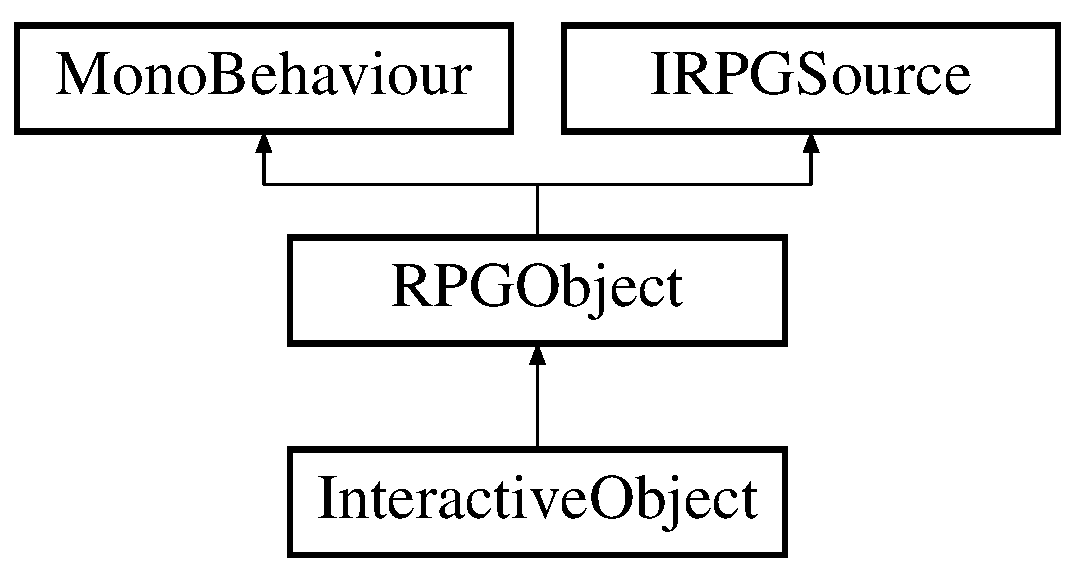
\includegraphics[height=3.000000cm]{class_interactive_object}
\end{center}
\end{figure}
\subsection*{Public Member Functions}
\begin{DoxyCompactItemize}
\item 
\hypertarget{class_interactive_object_abddd2865d50c231e21c2729c26d6466c}{}override bool {\bfseries Is\+Visible} (out int Hide\+Value, out \hyperlink{class_t_effect}{T\+Effect}\mbox{[}$\,$\mbox{]} Use\+Effects)\label{class_interactive_object_abddd2865d50c231e21c2729c26d6466c}

\item 
\hypertarget{class_interactive_object_a28ab335d2f20a2787a6ca2d91511552d}{}override bool {\bfseries Check\+Value} (string Name\+Of\+Value, out int Base\+Value, out int End\+Value, out \hyperlink{class_t_effect}{T\+Effect}\mbox{[}$\,$\mbox{]} Use\+Effects)\label{class_interactive_object_a28ab335d2f20a2787a6ca2d91511552d}

\item 
\hypertarget{class_interactive_object_af7977dcb81d6bc5a8714e5ade8013ae8}{}override float {\bfseries Recieve\+Damage} (float Value, string Typ)\label{class_interactive_object_af7977dcb81d6bc5a8714e5ade8013ae8}

\end{DoxyCompactItemize}
\subsection*{Additional Inherited Members}


The documentation for this class was generated from the following file\+:\begin{DoxyCompactItemize}
\item 
C\+:/\+Users/\+Jordan Eichner/\+Documents/\+Unity/\+Top\+Down\+R\+P\+G/\+Assets/\+Standard\+Assets/\+R\+P\+G-\/\+Sources/\+Scripts/\+Interactive\+Objects/Interactive\+Object.\+cs\end{DoxyCompactItemize}

\hypertarget{interface_i_r_p_g_source}{}\section{I\+R\+P\+G\+Source Interface Reference}
\label{interface_i_r_p_g_source}\index{I\+R\+P\+G\+Source@{I\+R\+P\+G\+Source}}
Inheritance diagram for I\+R\+P\+G\+Source\+:\begin{figure}[H]
\begin{center}
\leavevmode
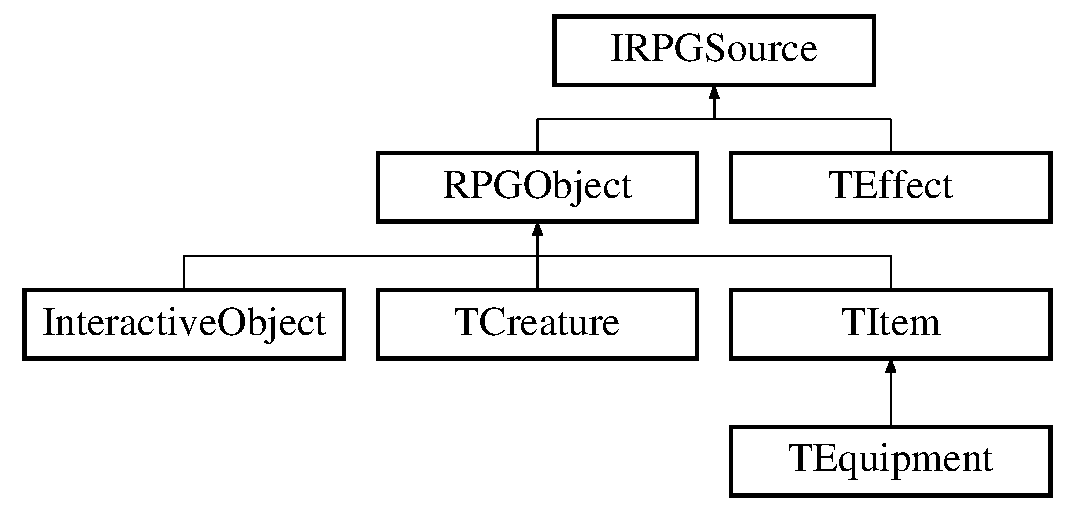
\includegraphics[height=4.000000cm]{interface_i_r_p_g_source}
\end{center}
\end{figure}
\subsection*{Public Member Functions}
\begin{DoxyCompactItemize}
\item 
\hypertarget{interface_i_r_p_g_source_a9d5a239ec9c77a2a462541257ab2dd08}{}void {\bfseries Send\+Message} (string Message, \hyperlink{interface_i_r_p_g_source}{I\+R\+P\+G\+Source} Source)\label{interface_i_r_p_g_source_a9d5a239ec9c77a2a462541257ab2dd08}

\end{DoxyCompactItemize}


The documentation for this interface was generated from the following file\+:\begin{DoxyCompactItemize}
\item 
C\+:/\+Users/\+Jordan Eichner/\+Documents/\+Unity/\+Top\+Down\+R\+P\+G/\+Assets/\+Standard\+Assets/\+R\+P\+G-\/\+Sources/\+Scripts/\+Meta/I\+R\+P\+G\+Source.\+cs\end{DoxyCompactItemize}

\hypertarget{class_r_p_g_object_1_1_attribut_modification_helper_1_1_modification}{}\section{R\+P\+G\+Object.\+Attribut\+Modification\+Helper.\+Modification Class Reference}
\label{class_r_p_g_object_1_1_attribut_modification_helper_1_1_modification}\index{R\+P\+G\+Object.\+Attribut\+Modification\+Helper.\+Modification@{R\+P\+G\+Object.\+Attribut\+Modification\+Helper.\+Modification}}
\subsection*{Public Member Functions}
\begin{DoxyCompactItemize}
\item 
\hypertarget{class_r_p_g_object_1_1_attribut_modification_helper_1_1_modification_af5220719b5d5a37d3d3d3383ad54c5a4}{}bool {\bfseries Is\+Supressed} (string Name)\label{class_r_p_g_object_1_1_attribut_modification_helper_1_1_modification_af5220719b5d5a37d3d3d3383ad54c5a4}

\item 
\hypertarget{class_r_p_g_object_1_1_attribut_modification_helper_1_1_modification_afa6572bc4595f877a06bb6c5d7d1863c}{}{\bfseries Modification} (string sourcetype, float value, int order, bool mode, \hyperlink{class_t_effect}{T\+Effect} sourceeffect)\label{class_r_p_g_object_1_1_attribut_modification_helper_1_1_modification_afa6572bc4595f877a06bb6c5d7d1863c}

\end{DoxyCompactItemize}
\subsection*{Public Attributes}
\begin{DoxyCompactItemize}
\item 
\hypertarget{class_r_p_g_object_1_1_attribut_modification_helper_1_1_modification_a209f4406dff4c1139b883f437c838c97}{}string {\bfseries Source\+Type}\label{class_r_p_g_object_1_1_attribut_modification_helper_1_1_modification_a209f4406dff4c1139b883f437c838c97}

\item 
\hypertarget{class_r_p_g_object_1_1_attribut_modification_helper_1_1_modification_ac47bbc3b20ca8250893a20e816feecd1}{}float {\bfseries Value}\label{class_r_p_g_object_1_1_attribut_modification_helper_1_1_modification_ac47bbc3b20ca8250893a20e816feecd1}

\item 
\hypertarget{class_r_p_g_object_1_1_attribut_modification_helper_1_1_modification_a5cab54c13609d00e3a0963aecf29109b}{}int {\bfseries Order}\label{class_r_p_g_object_1_1_attribut_modification_helper_1_1_modification_a5cab54c13609d00e3a0963aecf29109b}

\item 
\hypertarget{class_r_p_g_object_1_1_attribut_modification_helper_1_1_modification_ad4e4f83e54f7b0fec528d815c2cfc847}{}bool {\bfseries Mode}\label{class_r_p_g_object_1_1_attribut_modification_helper_1_1_modification_ad4e4f83e54f7b0fec528d815c2cfc847}

\item 
\hypertarget{class_r_p_g_object_1_1_attribut_modification_helper_1_1_modification_a096613a99f591c94f53e96bc31c20f73}{}\hyperlink{class_t_effect}{T\+Effect} {\bfseries Source\+Effect}\label{class_r_p_g_object_1_1_attribut_modification_helper_1_1_modification_a096613a99f591c94f53e96bc31c20f73}

\end{DoxyCompactItemize}


The documentation for this class was generated from the following file\+:\begin{DoxyCompactItemize}
\item 
C\+:/\+Users/\+Jordan Eichner/\+Documents/\+Unity/\+Top\+Down\+R\+P\+G/\+Assets/\+Standard\+Assets/\+R\+P\+G-\/\+Sources/\+Scripts/\+Meta/R\+P\+G\+Object.\+cs\end{DoxyCompactItemize}

\hypertarget{class_effect_script_object_1_1_numeric_value}{}\section{Effect\+Script\+Object.\+Numeric\+Value Class Reference}
\label{class_effect_script_object_1_1_numeric_value}\index{Effect\+Script\+Object.\+Numeric\+Value@{Effect\+Script\+Object.\+Numeric\+Value}}
\subsection*{Public Member Functions}
\begin{DoxyCompactItemize}
\item 
\hypertarget{class_effect_script_object_1_1_numeric_value_a16eae89225efd79f25f35d27537fd2c8}{}{\bfseries Numeric\+Value} (string name, float value)\label{class_effect_script_object_1_1_numeric_value_a16eae89225efd79f25f35d27537fd2c8}

\end{DoxyCompactItemize}
\subsection*{Public Attributes}
\begin{DoxyCompactItemize}
\item 
\hypertarget{class_effect_script_object_1_1_numeric_value_a999741e2fc10ebbcc4b09c0c396aebd3}{}string {\bfseries Name}\label{class_effect_script_object_1_1_numeric_value_a999741e2fc10ebbcc4b09c0c396aebd3}

\item 
\hypertarget{class_effect_script_object_1_1_numeric_value_a22b9e6b3ab3b960e7c9f2db374e77a30}{}float {\bfseries Value}\label{class_effect_script_object_1_1_numeric_value_a22b9e6b3ab3b960e7c9f2db374e77a30}

\end{DoxyCompactItemize}


The documentation for this class was generated from the following file\+:\begin{DoxyCompactItemize}
\item 
C\+:/\+Users/\+Jordan Eichner/\+Documents/\+Git\+Hub/\+Top\+Down\+R\+P\+G/\+Top\+Down\+R\+P\+G/\+Assets/\+Standard\+Assets/\+R\+P\+G libary/\+Scripts/\+Effects/Effect\+Script\+Object.\+cs\end{DoxyCompactItemize}

\hypertarget{class_r_p_g_object_1_1_numeric_value_helper}{}\section{R\+P\+G\+Object.\+Numeric\+Value\+Helper Class Reference}
\label{class_r_p_g_object_1_1_numeric_value_helper}\index{R\+P\+G\+Object.\+Numeric\+Value\+Helper@{R\+P\+G\+Object.\+Numeric\+Value\+Helper}}
Inheritance diagram for R\+P\+G\+Object.\+Numeric\+Value\+Helper\+:\begin{figure}[H]
\begin{center}
\leavevmode
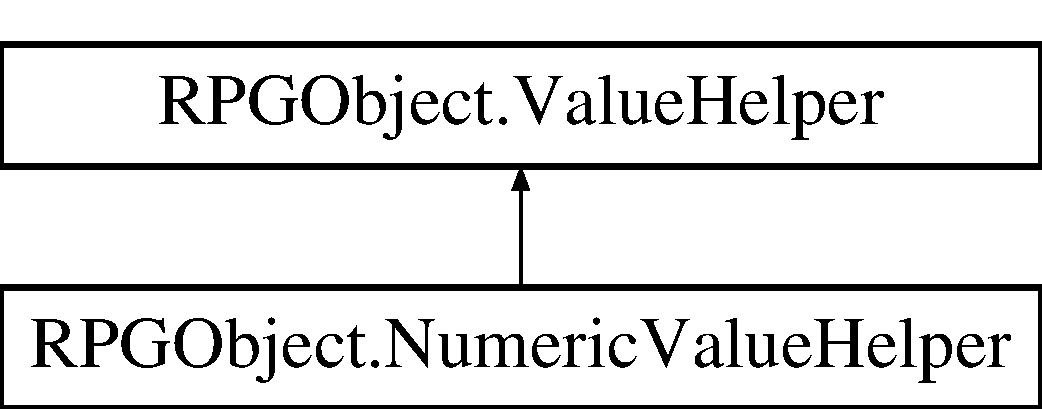
\includegraphics[height=2.000000cm]{class_r_p_g_object_1_1_numeric_value_helper}
\end{center}
\end{figure}
\subsection*{Public Attributes}
\begin{DoxyCompactItemize}
\item 
float \hyperlink{class_r_p_g_object_1_1_numeric_value_helper_a848b98b34e4029244f2764a8b1724704}{Value}
\end{DoxyCompactItemize}


\subsection{Detailed Description}
Spezialiesierte Hilfsklasse um Numerische(float) Werte zu speichern. 

\subsection{Member Data Documentation}
\hypertarget{class_r_p_g_object_1_1_numeric_value_helper_a848b98b34e4029244f2764a8b1724704}{}\index{R\+P\+G\+Object\+::\+Numeric\+Value\+Helper@{R\+P\+G\+Object\+::\+Numeric\+Value\+Helper}!Value@{Value}}
\index{Value@{Value}!R\+P\+G\+Object\+::\+Numeric\+Value\+Helper@{R\+P\+G\+Object\+::\+Numeric\+Value\+Helper}}
\subsubsection[{Value}]{\setlength{\rightskip}{0pt plus 5cm}float R\+P\+G\+Object.\+Numeric\+Value\+Helper.\+Value}\label{class_r_p_g_object_1_1_numeric_value_helper_a848b98b34e4029244f2764a8b1724704}
Naja der dem Namen zugeordnete Standard-\/\+Wert 

The documentation for this class was generated from the following file\+:\begin{DoxyCompactItemize}
\item 
C\+:/\+Users/\+Jordan Eichner/\+Documents/\+Git\+Hub/\+Top\+Down\+R\+P\+G/\+Top\+Down\+R\+P\+G/\+Assets/\+Standard\+Assets/\+R\+P\+G libary/\+Scripts/\+Meta/R\+P\+G\+Object.\+cs\end{DoxyCompactItemize}

\hypertarget{struct_effect_script_object_1_1_paramter}{}\section{Effect\+Script\+Object.\+Paramter Struct Reference}
\label{struct_effect_script_object_1_1_paramter}\index{Effect\+Script\+Object.\+Paramter@{Effect\+Script\+Object.\+Paramter}}
\subsection*{Public Member Functions}
\begin{DoxyCompactItemize}
\item 
\hypertarget{struct_effect_script_object_1_1_paramter_a4976df3086256963524914b441684202}{}{\bfseries Paramter} (string \+\_\+\+Name, object \+\_\+\+O)\label{struct_effect_script_object_1_1_paramter_a4976df3086256963524914b441684202}

\end{DoxyCompactItemize}
\subsection*{Public Attributes}
\begin{DoxyCompactItemize}
\item 
\hypertarget{struct_effect_script_object_1_1_paramter_ac64c1d743c49f514f3b9eed444743ca0}{}string {\bfseries Name}\label{struct_effect_script_object_1_1_paramter_ac64c1d743c49f514f3b9eed444743ca0}

\item 
\hypertarget{struct_effect_script_object_1_1_paramter_ae53d84d7ec439dcc27230b13d487c203}{}object {\bfseries O}\label{struct_effect_script_object_1_1_paramter_ae53d84d7ec439dcc27230b13d487c203}

\end{DoxyCompactItemize}


The documentation for this struct was generated from the following file\+:\begin{DoxyCompactItemize}
\item 
C\+:/\+Users/\+Jordan Eichner/\+Documents/\+Unity/\+Top\+Down\+R\+P\+G/\+Assets/\+Standard\+Assets/\+R\+P\+G-\/\+Sources/\+Scripts/\+Effects/Effect\+Script\+Object.\+cs\end{DoxyCompactItemize}

\hypertarget{class_r_p_g_object}{}\section{R\+P\+G\+Object Class Reference}
\label{class_r_p_g_object}\index{R\+P\+G\+Object@{R\+P\+G\+Object}}


Diese Basisklasse vereinheitlicht die wichtigsten Eigenschaften aller Objekte, die Teil der vom R\+P\+G-\/\+System verwalteten Welt sind.  


Inheritance diagram for R\+P\+G\+Object\+:\begin{figure}[H]
\begin{center}
\leavevmode
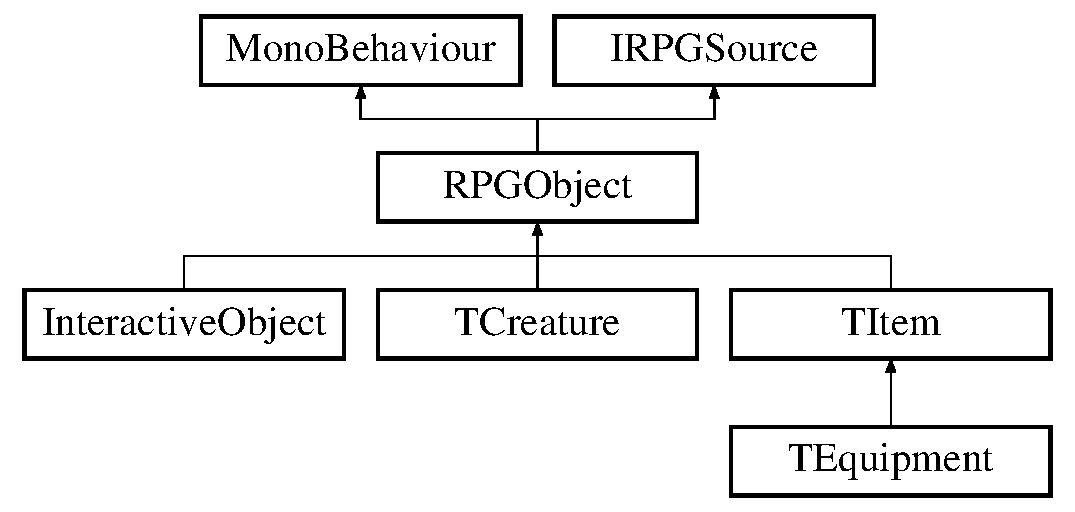
\includegraphics[height=4.000000cm]{class_r_p_g_object}
\end{center}
\end{figure}
\subsection*{Classes}
\begin{DoxyCompactItemize}
\item 
class \hyperlink{class_r_p_g_object_1_1_attribut_modification_helper}{Attribut\+Modification\+Helper}
\item 
class \hyperlink{class_r_p_g_object_1_1boolean_value_helper}{boolean\+Value\+Helper}
\item 
class \hyperlink{class_r_p_g_object_1_1_numeric_value_helper}{Numeric\+Value\+Helper}
\item 
class \hyperlink{class_r_p_g_object_1_1_value_helper}{Value\+Helper}
\end{DoxyCompactItemize}
\subsection*{Public Member Functions}
\begin{DoxyCompactItemize}
\item 
\hypertarget{class_r_p_g_object_adf3b238298fba6c2c3551102b042699d}{}virtual bool {\bfseries Add\+Effect} (\hyperlink{class_t_effect}{T\+Effect} Effect)\label{class_r_p_g_object_adf3b238298fba6c2c3551102b042699d}

\item 
\hypertarget{class_r_p_g_object_abbb053e8e6cbcd036d3ae91a1d593720}{}virtual string\mbox{[}$\,$\mbox{]} {\bfseries Get\+Information} (\hyperlink{class_r_p_g_object}{R\+P\+G\+Object} Sender, bool Is\+Deep\+Search=false)\label{class_r_p_g_object_abbb053e8e6cbcd036d3ae91a1d593720}

\item 
\hypertarget{class_r_p_g_object_a931b4ce1cf1e97c803438f70e10c8784}{}void {\bfseries Update\+Effects} (float timestep)\label{class_r_p_g_object_a931b4ce1cf1e97c803438f70e10c8784}

\item 
\hypertarget{class_r_p_g_object_a870001224da5b930a8903c83929c162f}{}abstract bool {\bfseries Is\+Visible} (out int Hide\+Value, out \hyperlink{class_t_effect}{T\+Effect}\mbox{[}$\,$\mbox{]} Use\+Effects)\label{class_r_p_g_object_a870001224da5b930a8903c83929c162f}

\item 
\hypertarget{class_r_p_g_object_ad35719a061adfae0dd43f343aceab73b}{}abstract bool {\bfseries Check\+Value} (string Name\+Of\+Value, out int Base\+Value, out int End\+Value, out \hyperlink{class_t_effect}{T\+Effect}\mbox{[}$\,$\mbox{]} Use\+Effects)\label{class_r_p_g_object_ad35719a061adfae0dd43f343aceab73b}

\item 
\hypertarget{class_r_p_g_object_ace0438534a4b8d6efa00a08ae6fab68b}{}abstract float {\bfseries Recieve\+Damage} (float Value, string Typ)\label{class_r_p_g_object_ace0438534a4b8d6efa00a08ae6fab68b}

\end{DoxyCompactItemize}
\subsection*{Protected Member Functions}
\begin{DoxyCompactItemize}
\item 
\hypertarget{class_r_p_g_object_ab05437a7714f58d52ee610f1fb9c052b}{}float {\bfseries Get\+N\+Base\+Value} (string Name)\label{class_r_p_g_object_ab05437a7714f58d52ee610f1fb9c052b}

\item 
\hypertarget{class_r_p_g_object_a7772162c56eed453f9f97b6ac01bc48b}{}bool {\bfseries Get\+B\+Base\+Value} (string Name)\label{class_r_p_g_object_a7772162c56eed453f9f97b6ac01bc48b}

\item 
\hypertarget{class_r_p_g_object_a766f2912c7947d76a429a373b3073ce2}{}void {\bfseries On\+New\+Effect} (\hyperlink{class_t_effect}{T\+Effect} effect)\label{class_r_p_g_object_a766f2912c7947d76a429a373b3073ce2}

\item 
\hypertarget{class_r_p_g_object_a3c97b73354e9eec8e3ad5d85308ba728}{}void {\bfseries On\+Remove\+Effect} (\hyperlink{class_t_effect}{T\+Effect} effect)\label{class_r_p_g_object_a3c97b73354e9eec8e3ad5d85308ba728}

\item 
\hypertarget{class_r_p_g_object_af344332996644a20d6a3b87d8c22b89f}{}void {\bfseries Enforce\+Effect\+Supression} ()\label{class_r_p_g_object_af344332996644a20d6a3b87d8c22b89f}

\item 
\hypertarget{class_r_p_g_object_a4480d28e80d2f5d59c0b831817c74621}{}float {\bfseries Get\+Current\+Value\+Modification} (string Name)\label{class_r_p_g_object_a4480d28e80d2f5d59c0b831817c74621}

\item 
\hypertarget{class_r_p_g_object_a548b39ae1ef3c7084662289fc801101c}{}virtual void {\bfseries Update\+Statistics} ()\label{class_r_p_g_object_a548b39ae1ef3c7084662289fc801101c}

\item 
\hypertarget{class_r_p_g_object_a6b796a1ff13ea340a81690ee81d62848}{}abstract float {\bfseries Recieve\+Healing} (float Value)\label{class_r_p_g_object_a6b796a1ff13ea340a81690ee81d62848}

\end{DoxyCompactItemize}
\subsection*{Protected Attributes}
\begin{DoxyCompactItemize}
\item 
float \hyperlink{class_r_p_g_object_a550507f127d2915aa0b7a95ef5e3feb6}{b\+Weight}
\item 
float \hyperlink{class_r_p_g_object_a098dcfa4772557888348f5164da509f8}{c\+Weight}
\item 
Size\+Category \hyperlink{class_r_p_g_object_ae5cb76ccbe4f37237cc03a9737009577}{b\+Size\+Category}
\item 
Size\+Category \hyperlink{class_r_p_g_object_a5076aeba98770e8507778eb6051df87b}{c\+Size\+Category}
\item 
List$<$ \hyperlink{class_t_effect}{T\+Effect} $>$ \hyperlink{class_r_p_g_object_a833cf33788a1040a7fdcb703d6e3126d}{c\+Effects} = new List$<$\hyperlink{class_t_effect}{T\+Effect}$>$ ()
\item 
List$<$ \hyperlink{struct_content}{Content} $>$ \hyperlink{class_r_p_g_object_ac5b133eca19e8f97988722018cdf139b}{c\+Information} = new List$<$\hyperlink{struct_content}{Content}$>$ ()
\item 
\hypertarget{class_r_p_g_object_aca7f376707b78c0852b0001ee67dc80f}{}List$<$ \hyperlink{class_r_p_g_object_1_1_value_helper}{Value\+Helper} $>$ {\bfseries b\+Values} =new List$<$\hyperlink{class_r_p_g_object_1_1_value_helper}{Value\+Helper}$>$()\label{class_r_p_g_object_aca7f376707b78c0852b0001ee67dc80f}

\item 
\hypertarget{class_r_p_g_object_a19aea805ab96ccaa5bd202bebe6ff482}{}List$<$ \hyperlink{class_r_p_g_object_1_1_attribut_modification_helper}{Attribut\+Modification\+Helper} $>$ {\bfseries Attribute\+Helper} = new List$<$\hyperlink{class_r_p_g_object_1_1_attribut_modification_helper}{Attribut\+Modification\+Helper}$>$ ()\label{class_r_p_g_object_a19aea805ab96ccaa5bd202bebe6ff482}

\end{DoxyCompactItemize}
\subsection*{Properties}
\begin{DoxyCompactItemize}
\item 
virtual Size\+Category \hyperlink{class_r_p_g_object_ad4fe72a3a4621618a563219805ede17d}{Size}\hspace{0.3cm}{\ttfamily  \mbox{[}get\mbox{]}}
\item 
virtual List$<$ \hyperlink{class_t_effect}{T\+Effect} $>$ \hyperlink{class_r_p_g_object_ac13bdb9e5988e9eff18e5f6f5b613bb6}{Effects}\hspace{0.3cm}{\ttfamily  \mbox{[}get\mbox{]}}
\item 
virtual float \hyperlink{class_r_p_g_object_af627383d88885ca597a549cb52e4b242}{Weight}\hspace{0.3cm}{\ttfamily  \mbox{[}get\mbox{]}}
\item 
\hypertarget{class_r_p_g_object_a312d68adaf6a8eb15319d3cac8198802}{}virtual List$<$ \hyperlink{struct_content}{Content} $>$ {\bfseries Information}\hspace{0.3cm}{\ttfamily  \mbox{[}get\mbox{]}}\label{class_r_p_g_object_a312d68adaf6a8eb15319d3cac8198802}

\end{DoxyCompactItemize}


\subsection{Detailed Description}
Diese Basisklasse vereinheitlicht die wichtigsten Eigenschaften aller Objekte, die Teil der vom R\+P\+G-\/\+System verwalteten Welt sind. 

\begin{DoxyAuthor}{Author}
Jordan Eichner 
\end{DoxyAuthor}


\subsection{Member Data Documentation}
\hypertarget{class_r_p_g_object_ae5cb76ccbe4f37237cc03a9737009577}{}\index{R\+P\+G\+Object@{R\+P\+G\+Object}!b\+Size\+Category@{b\+Size\+Category}}
\index{b\+Size\+Category@{b\+Size\+Category}!R\+P\+G\+Object@{R\+P\+G\+Object}}
\subsubsection[{b\+Size\+Category}]{\setlength{\rightskip}{0pt plus 5cm}Size\+Category R\+P\+G\+Object.\+b\+Size\+Category\hspace{0.3cm}{\ttfamily [protected]}}\label{class_r_p_g_object_ae5cb76ccbe4f37237cc03a9737009577}
Größenordnung für Modifikationen \hypertarget{class_r_p_g_object_a550507f127d2915aa0b7a95ef5e3feb6}{}\index{R\+P\+G\+Object@{R\+P\+G\+Object}!b\+Weight@{b\+Weight}}
\index{b\+Weight@{b\+Weight}!R\+P\+G\+Object@{R\+P\+G\+Object}}
\subsubsection[{b\+Weight}]{\setlength{\rightskip}{0pt plus 5cm}float R\+P\+G\+Object.\+b\+Weight\hspace{0.3cm}{\ttfamily [protected]}}\label{class_r_p_g_object_a550507f127d2915aa0b7a95ef5e3feb6}
Standardgewicht in kg in einer Umgebung mit Standard g; \hypertarget{class_r_p_g_object_a833cf33788a1040a7fdcb703d6e3126d}{}\index{R\+P\+G\+Object@{R\+P\+G\+Object}!c\+Effects@{c\+Effects}}
\index{c\+Effects@{c\+Effects}!R\+P\+G\+Object@{R\+P\+G\+Object}}
\subsubsection[{c\+Effects}]{\setlength{\rightskip}{0pt plus 5cm}List$<${\bf T\+Effect}$>$ R\+P\+G\+Object.\+c\+Effects = new List$<${\bf T\+Effect}$>$ ()\hspace{0.3cm}{\ttfamily [protected]}}\label{class_r_p_g_object_a833cf33788a1040a7fdcb703d6e3126d}
Geschützte Liste für Effekte ist über die entsprechenden Funktionen(\+Add\+Efect,\+Remove\+Effect) von außen aufzurufen \hypertarget{class_r_p_g_object_ac5b133eca19e8f97988722018cdf139b}{}\index{R\+P\+G\+Object@{R\+P\+G\+Object}!c\+Information@{c\+Information}}
\index{c\+Information@{c\+Information}!R\+P\+G\+Object@{R\+P\+G\+Object}}
\subsubsection[{c\+Information}]{\setlength{\rightskip}{0pt plus 5cm}List$<${\bf Content}$>$ R\+P\+G\+Object.\+c\+Information = new List$<${\bf Content}$>$ ()\hspace{0.3cm}{\ttfamily [protected]}}\label{class_r_p_g_object_ac5b133eca19e8f97988722018cdf139b}
Liste von Informationen. \hypertarget{class_r_p_g_object_a5076aeba98770e8507778eb6051df87b}{}\index{R\+P\+G\+Object@{R\+P\+G\+Object}!c\+Size\+Category@{c\+Size\+Category}}
\index{c\+Size\+Category@{c\+Size\+Category}!R\+P\+G\+Object@{R\+P\+G\+Object}}
\subsubsection[{c\+Size\+Category}]{\setlength{\rightskip}{0pt plus 5cm}Size\+Category R\+P\+G\+Object.\+c\+Size\+Category\hspace{0.3cm}{\ttfamily [protected]}}\label{class_r_p_g_object_a5076aeba98770e8507778eb6051df87b}
Durch Effekte veränderte Größe \hypertarget{class_r_p_g_object_a098dcfa4772557888348f5164da509f8}{}\index{R\+P\+G\+Object@{R\+P\+G\+Object}!c\+Weight@{c\+Weight}}
\index{c\+Weight@{c\+Weight}!R\+P\+G\+Object@{R\+P\+G\+Object}}
\subsubsection[{c\+Weight}]{\setlength{\rightskip}{0pt plus 5cm}float R\+P\+G\+Object.\+c\+Weight\hspace{0.3cm}{\ttfamily [protected]}}\label{class_r_p_g_object_a098dcfa4772557888348f5164da509f8}
Durch Effekte verändertes Gewicht 

\subsection{Property Documentation}
\hypertarget{class_r_p_g_object_ac13bdb9e5988e9eff18e5f6f5b613bb6}{}\index{R\+P\+G\+Object@{R\+P\+G\+Object}!Effects@{Effects}}
\index{Effects@{Effects}!R\+P\+G\+Object@{R\+P\+G\+Object}}
\subsubsection[{Effects}]{\setlength{\rightskip}{0pt plus 5cm}virtual List$<${\bf T\+Effect}$>$ R\+P\+G\+Object.\+Effects\hspace{0.3cm}{\ttfamily [get]}}\label{class_r_p_g_object_ac13bdb9e5988e9eff18e5f6f5b613bb6}
Öffentliche Eigenschaft zum Auslesen aller Effekte, die auf das Objekt einwirken \hypertarget{class_r_p_g_object_ad4fe72a3a4621618a563219805ede17d}{}\index{R\+P\+G\+Object@{R\+P\+G\+Object}!Size@{Size}}
\index{Size@{Size}!R\+P\+G\+Object@{R\+P\+G\+Object}}
\subsubsection[{Size}]{\setlength{\rightskip}{0pt plus 5cm}virtual Size\+Category R\+P\+G\+Object.\+Size\hspace{0.3cm}{\ttfamily [get]}}\label{class_r_p_g_object_ad4fe72a3a4621618a563219805ede17d}
Öffentliche Eigenschaft zum Auslesen der aktuelle Größenordnung \hypertarget{class_r_p_g_object_af627383d88885ca597a549cb52e4b242}{}\index{R\+P\+G\+Object@{R\+P\+G\+Object}!Weight@{Weight}}
\index{Weight@{Weight}!R\+P\+G\+Object@{R\+P\+G\+Object}}
\subsubsection[{Weight}]{\setlength{\rightskip}{0pt plus 5cm}virtual float R\+P\+G\+Object.\+Weight\hspace{0.3cm}{\ttfamily [get]}}\label{class_r_p_g_object_af627383d88885ca597a549cb52e4b242}
Öffentliche Eigenschaft zum Auslesen des aktuellen Gewichts 

The documentation for this class was generated from the following file\+:\begin{DoxyCompactItemize}
\item 
C\+:/\+Users/\+Jordan Eichner/\+Documents/\+Unity/\+Top\+Down\+R\+P\+G/\+Assets/\+Standard\+Assets/\+R\+P\+G-\/\+Sources/\+Scripts/\+Meta/R\+P\+G\+Object.\+cs\end{DoxyCompactItemize}

\hypertarget{class_effect_script_object_1_1_string_value}{}\section{Effect\+Script\+Object.\+String\+Value Class Reference}
\label{class_effect_script_object_1_1_string_value}\index{Effect\+Script\+Object.\+String\+Value@{Effect\+Script\+Object.\+String\+Value}}
\subsection*{Public Member Functions}
\begin{DoxyCompactItemize}
\item 
\hypertarget{class_effect_script_object_1_1_string_value_afc4b7dd444e28462edd5d2796d736b98}{}{\bfseries String\+Value} (string name, string value)\label{class_effect_script_object_1_1_string_value_afc4b7dd444e28462edd5d2796d736b98}

\end{DoxyCompactItemize}
\subsection*{Public Attributes}
\begin{DoxyCompactItemize}
\item 
\hypertarget{class_effect_script_object_1_1_string_value_ae654f4ac63b2a53d82b857b77e3c23ca}{}string {\bfseries Name}\label{class_effect_script_object_1_1_string_value_ae654f4ac63b2a53d82b857b77e3c23ca}

\item 
\hypertarget{class_effect_script_object_1_1_string_value_a14dc217e730e132de31929bc718dd2e6}{}string {\bfseries Value}\label{class_effect_script_object_1_1_string_value_a14dc217e730e132de31929bc718dd2e6}

\end{DoxyCompactItemize}


The documentation for this class was generated from the following file\+:\begin{DoxyCompactItemize}
\item 
C\+:/\+Users/\+Jordan Eichner/\+Documents/\+Unity/\+Top\+Down\+R\+P\+G/\+Assets/\+Standard\+Assets/\+R\+P\+G-\/\+Sources/\+Scripts/\+Effects/Effect\+Script\+Object.\+cs\end{DoxyCompactItemize}

\hypertarget{class_t_creature}{}\section{T\+Creature Class Reference}
\label{class_t_creature}\index{T\+Creature@{T\+Creature}}
Inheritance diagram for T\+Creature\+:\begin{figure}[H]
\begin{center}
\leavevmode
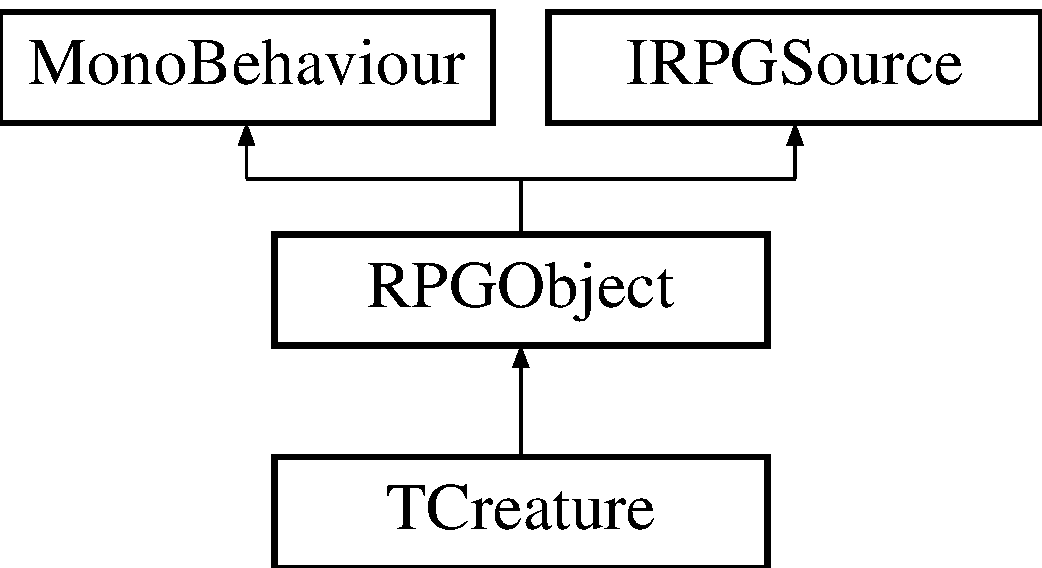
\includegraphics[height=3.000000cm]{class_t_creature}
\end{center}
\end{figure}
\subsection*{Classes}
\begin{DoxyCompactItemize}
\item 
struct \hyperlink{struct_t_creature_1_1_equipment_slot}{Equipment\+Slot}
\item 
class \hyperlink{class_t_creature_1_1_skill}{Skill}
\begin{DoxyCompactList}\small\item\em Klasse zum bereitstellen von Talentinformationen. \end{DoxyCompactList}\end{DoxyCompactItemize}
\subsection*{Public Member Functions}
\begin{DoxyCompactItemize}
\item 
\hypertarget{class_t_creature_ab49e4ba9805e8ea34ed2992f5b9eb507}{}override bool {\bfseries Is\+Visible} (out int Hide\+Value, out \hyperlink{class_t_effect}{T\+Effect}\mbox{[}$\,$\mbox{]} Use\+Effects)\label{class_t_creature_ab49e4ba9805e8ea34ed2992f5b9eb507}

\item 
\hypertarget{class_t_creature_a721027f6e2ddb18cc24617da081d609b}{}override bool {\bfseries Check\+Value} (string Name\+Of\+Value, out int Base\+Value, out int End\+Value, out \hyperlink{class_t_effect}{T\+Effect}\mbox{[}$\,$\mbox{]} Use\+Effects)\label{class_t_creature_a721027f6e2ddb18cc24617da081d609b}

\item 
\hypertarget{class_t_creature_a875491187fd013158f76ac0f11de9506}{}override float {\bfseries Recieve\+Damage} (float Value, string Typ)\label{class_t_creature_a875491187fd013158f76ac0f11de9506}

\end{DoxyCompactItemize}
\subsection*{Protected Member Functions}
\begin{DoxyCompactItemize}
\item 
\hypertarget{class_t_creature_a8126c06e7c10d622826dcd165743aa66}{}override void {\bfseries Update\+Statistics} ()\label{class_t_creature_a8126c06e7c10d622826dcd165743aa66}

\item 
\hypertarget{class_t_creature_a7ecc901d6aaf6d0dca29e954909f0ba9}{}override float {\bfseries Recieve\+Healing} (float Value)\label{class_t_creature_a7ecc901d6aaf6d0dca29e954909f0ba9}

\end{DoxyCompactItemize}
\subsection*{Properties}
\begin{DoxyCompactItemize}
\item 
\hypertarget{class_t_creature_a470442b1fe4c9ffff515e1f434180bd4}{}override List$<$ \hyperlink{class_t_effect}{T\+Effect} $>$ {\bfseries Effects}\hspace{0.3cm}{\ttfamily  \mbox{[}get\mbox{]}}\label{class_t_creature_a470442b1fe4c9ffff515e1f434180bd4}

\item 
\hypertarget{class_t_creature_a4fe0cc004602abcfb355c0ee9b00434f}{}int {\bfseries Strength}\hspace{0.3cm}{\ttfamily  \mbox{[}get\mbox{]}}\label{class_t_creature_a4fe0cc004602abcfb355c0ee9b00434f}

\item 
\hypertarget{class_t_creature_acbfc87895abbbfe4a4aa0d79763ac827}{}int {\bfseries Dexterity}\hspace{0.3cm}{\ttfamily  \mbox{[}get\mbox{]}}\label{class_t_creature_acbfc87895abbbfe4a4aa0d79763ac827}

\item 
\hypertarget{class_t_creature_a8ff8e587b83f3bb665d26228ffaa200e}{}int {\bfseries Constitution}\hspace{0.3cm}{\ttfamily  \mbox{[}get\mbox{]}}\label{class_t_creature_a8ff8e587b83f3bb665d26228ffaa200e}

\item 
\hypertarget{class_t_creature_a439dc005b1ee3046dcadcf2c0a7c1fd0}{}int {\bfseries Metabolism}\hspace{0.3cm}{\ttfamily  \mbox{[}get\mbox{]}}\label{class_t_creature_a439dc005b1ee3046dcadcf2c0a7c1fd0}

\item 
\hypertarget{class_t_creature_afd9b5c88e8f45edfe6f1c9c8b9aac93c}{}int {\bfseries Intelligence}\hspace{0.3cm}{\ttfamily  \mbox{[}get\mbox{]}}\label{class_t_creature_afd9b5c88e8f45edfe6f1c9c8b9aac93c}

\item 
\hypertarget{class_t_creature_a74852b4ea525154ce9110643fc18ea5e}{}int {\bfseries Wisdom}\hspace{0.3cm}{\ttfamily  \mbox{[}get\mbox{]}}\label{class_t_creature_a74852b4ea525154ce9110643fc18ea5e}

\item 
\hypertarget{class_t_creature_abfd4d0ed1defc42cda03ee6b2057acaf}{}int {\bfseries Charisma}\hspace{0.3cm}{\ttfamily  \mbox{[}get\mbox{]}}\label{class_t_creature_abfd4d0ed1defc42cda03ee6b2057acaf}

\item 
\hypertarget{class_t_creature_ab7b3de27c987823c26de7ddde777965f}{}int {\bfseries Appearance}\hspace{0.3cm}{\ttfamily  \mbox{[}get\mbox{]}}\label{class_t_creature_ab7b3de27c987823c26de7ddde777965f}

\item 
\hypertarget{class_t_creature_aa66e0648f3eb3946247d65b253d3102d}{}override float {\bfseries this\mbox{[}string Value\+Name\mbox{]}}\hspace{0.3cm}{\ttfamily  \mbox{[}get\mbox{]}}\label{class_t_creature_aa66e0648f3eb3946247d65b253d3102d}

\item 
\hypertarget{class_t_creature_adcdd20275c79dc8b542e1c945135523f}{}bool {\bfseries this\mbox{[}string Value\+Name, int i\mbox{]}}\hspace{0.3cm}{\ttfamily  \mbox{[}get\mbox{]}}\label{class_t_creature_adcdd20275c79dc8b542e1c945135523f}

\item 
\hypertarget{class_t_creature_a4ee1294c6f08b7fa6e71ec3bc88694c1}{}List$<$ \hyperlink{struct_t_creature_1_1_equipment_slot}{Equipment\+Slot} $>$ {\bfseries Equipment}\hspace{0.3cm}{\ttfamily  \mbox{[}get\mbox{]}}\label{class_t_creature_a4ee1294c6f08b7fa6e71ec3bc88694c1}

\item 
\hypertarget{class_t_creature_a7aa47ddea4d58f4e205203861e46617c}{}List$<$ \hyperlink{class_t_item}{T\+Item} $>$ {\bfseries Inventory}\hspace{0.3cm}{\ttfamily  \mbox{[}get\mbox{]}}\label{class_t_creature_a7aa47ddea4d58f4e205203861e46617c}

\end{DoxyCompactItemize}
\subsection*{Additional Inherited Members}


The documentation for this class was generated from the following file\+:\begin{DoxyCompactItemize}
\item 
C\+:/\+Users/\+Jordan Eichner/\+Documents/\+Git\+Hub/\+Top\+Down\+R\+P\+G/\+Top\+Down\+R\+P\+G/\+Assets/\+Standard\+Assets/\+R\+P\+G libary/\+Scripts/\+Creatures/T\+Creature.\+cs\end{DoxyCompactItemize}

\hypertarget{class_t_effect}{}\section{T\+Effect Class Reference}
\label{class_t_effect}\index{T\+Effect@{T\+Effect}}
Inheritance diagram for T\+Effect\+:\begin{figure}[H]
\begin{center}
\leavevmode
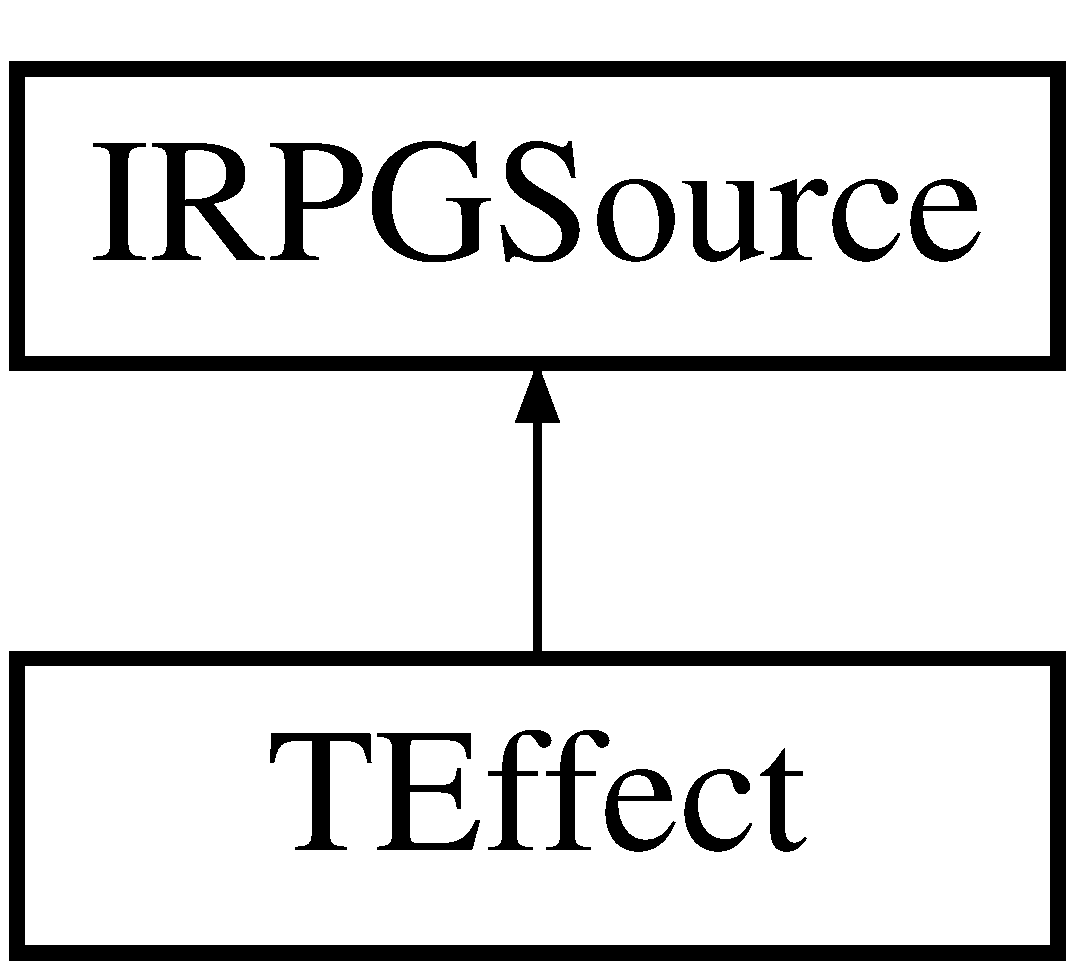
\includegraphics[height=2.000000cm]{class_t_effect}
\end{center}
\end{figure}
\subsection*{Public Attributes}
\begin{DoxyCompactItemize}
\item 
\hypertarget{class_t_effect_ae2e16fed884be48995efaa34fe1de953}{}string {\bfseries Name}\label{class_t_effect_ae2e16fed884be48995efaa34fe1de953}

\item 
\hypertarget{class_t_effect_af4c05ccaf01ff60830476692e664ed46}{}\hyperlink{interface_i_r_p_g_source}{I\+R\+P\+G\+Source} {\bfseries Original\+Source}\label{class_t_effect_af4c05ccaf01ff60830476692e664ed46}

\item 
\hypertarget{class_t_effect_a055eecd64b18735565edfca0038d2a63}{}\hyperlink{struct_content}{Content}\mbox{[}$\,$\mbox{]} {\bfseries Information}\label{class_t_effect_a055eecd64b18735565edfca0038d2a63}

\item 
\hypertarget{class_t_effect_a8d72bc042c7aa936103d7d9a1b73dbdd}{}string {\bfseries General\+Category}\label{class_t_effect_a8d72bc042c7aa936103d7d9a1b73dbdd}

\item 
\hypertarget{class_t_effect_a4e87f7bde97b87ab4d6b752188448d91}{}string {\bfseries Tags}\label{class_t_effect_a4e87f7bde97b87ab4d6b752188448d91}

\item 
\hypertarget{class_t_effect_a20680745c6f644fa9eef2437d68fa08f}{}int {\bfseries General\+Order}\label{class_t_effect_a20680745c6f644fa9eef2437d68fa08f}

\item 
\hypertarget{class_t_effect_adc77902a018f410d4dfeb4876e46d9b2}{}string\mbox{[}$\,$\mbox{]} {\bfseries Passive\+Effect\+Strings}\label{class_t_effect_adc77902a018f410d4dfeb4876e46d9b2}

\item 
\hypertarget{class_t_effect_a247fa858e50f50d3fc366e0b722ed7a0}{}List$<$ string $>$ {\bfseries Working\+Passive\+Effect\+Strings}\label{class_t_effect_a247fa858e50f50d3fc366e0b722ed7a0}

\item 
\hypertarget{class_t_effect_aadda58a14ce7f7c5565a6e35d1297ab9}{}string\mbox{[}$\,$\mbox{]} {\bfseries Active\+Effect\+Strings}\label{class_t_effect_aadda58a14ce7f7c5565a6e35d1297ab9}

\item 
\hypertarget{class_t_effect_ad829ee82d6cafadeb4c64ac6b089af87}{}string\mbox{[}$\,$\mbox{]} {\bfseries Reaction\+Effect\+Strings}\label{class_t_effect_ad829ee82d6cafadeb4c64ac6b089af87}

\item 
\hypertarget{class_t_effect_a7f399810b14063d6c6b0b610371716cf}{}bool {\bfseries Is\+Supressed}\label{class_t_effect_a7f399810b14063d6c6b0b610371716cf}

\item 
\hypertarget{class_t_effect_a3f8f5bc0e5f84245b3796f323d58972e}{}float {\bfseries o\+Duration}\label{class_t_effect_a3f8f5bc0e5f84245b3796f323d58972e}

\item 
\hypertarget{class_t_effect_a8c14995057021d94bf01d4821ff6534f}{}float {\bfseries c\+Duration}\label{class_t_effect_a8c14995057021d94bf01d4821ff6534f}

\end{DoxyCompactItemize}
\subsection*{Properties}
\begin{DoxyCompactItemize}
\item 
\hypertarget{class_t_effect_a5809fc4642f65d39a96e84eca3d16181}{}\hyperlink{class_effect_script_object}{Effect\+Script\+Object}\mbox{[}$\,$\mbox{]} {\bfseries Script\+Objects}\hspace{0.3cm}{\ttfamily  \mbox{[}get\mbox{]}}\label{class_t_effect_a5809fc4642f65d39a96e84eca3d16181}

\end{DoxyCompactItemize}
\subsection*{Additional Inherited Members}


The documentation for this class was generated from the following file\+:\begin{DoxyCompactItemize}
\item 
C\+:/\+Users/\+Jordan Eichner/\+Documents/\+Unity/\+Top\+Down\+R\+P\+G/\+Assets/\+Standard\+Assets/\+R\+P\+G-\/\+Sources/\+Scripts/\+Effects/T\+Effect.\+cs\end{DoxyCompactItemize}

\hypertarget{class_t_equipment}{}\section{T\+Equipment Class Reference}
\label{class_t_equipment}\index{T\+Equipment@{T\+Equipment}}
Inheritance diagram for T\+Equipment\+:\begin{figure}[H]
\begin{center}
\leavevmode
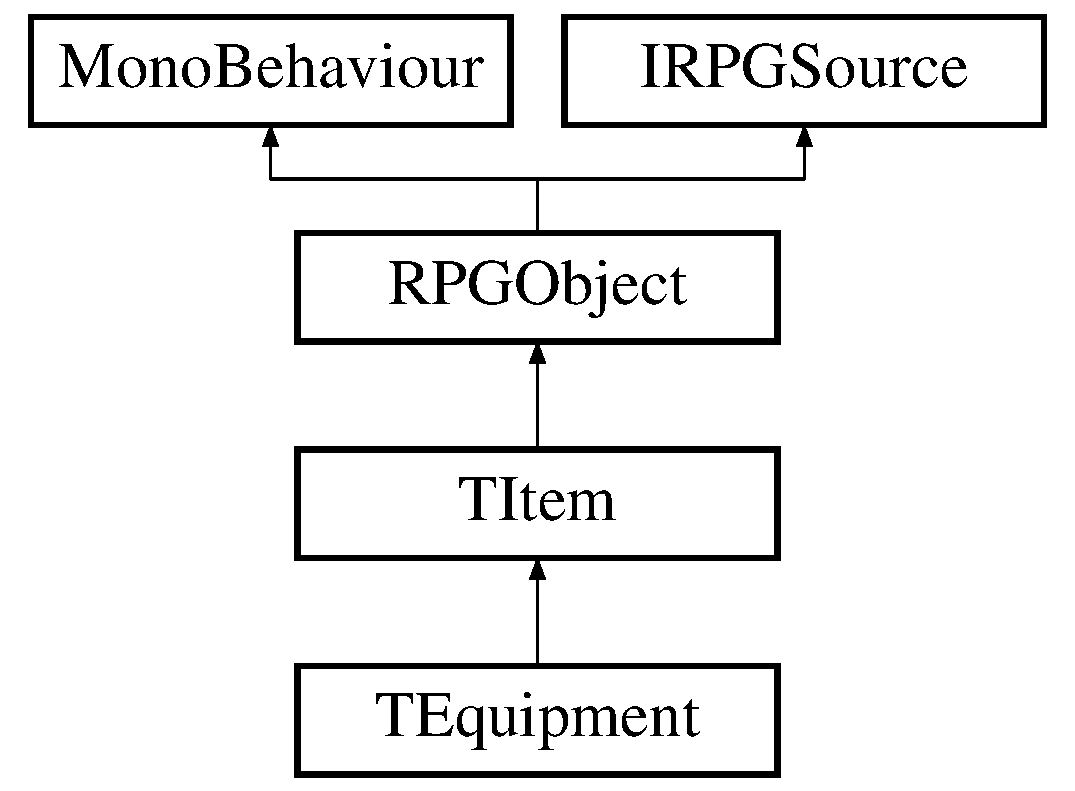
\includegraphics[height=4.000000cm]{class_t_equipment}
\end{center}
\end{figure}
\subsection*{Public Attributes}
\begin{DoxyCompactItemize}
\item 
\hypertarget{class_t_equipment_a0649573d41f70f840da2b3888af650b3}{}string {\bfseries Equipment\+Slot}\label{class_t_equipment_a0649573d41f70f840da2b3888af650b3}

\end{DoxyCompactItemize}
\subsection*{Additional Inherited Members}


The documentation for this class was generated from the following file\+:\begin{DoxyCompactItemize}
\item 
C\+:/\+Users/\+Jordan Eichner/\+Documents/\+Unity/\+Top\+Down\+R\+P\+G/\+Assets/\+Standard\+Assets/\+R\+P\+G-\/\+Sources/\+Scripts/\+Items/\+Equipment/T\+Equipment.\+cs\end{DoxyCompactItemize}

\hypertarget{class_t_item}{}\section{T\+Item Class Reference}
\label{class_t_item}\index{T\+Item@{T\+Item}}
Inheritance diagram for T\+Item\+:\begin{figure}[H]
\begin{center}
\leavevmode
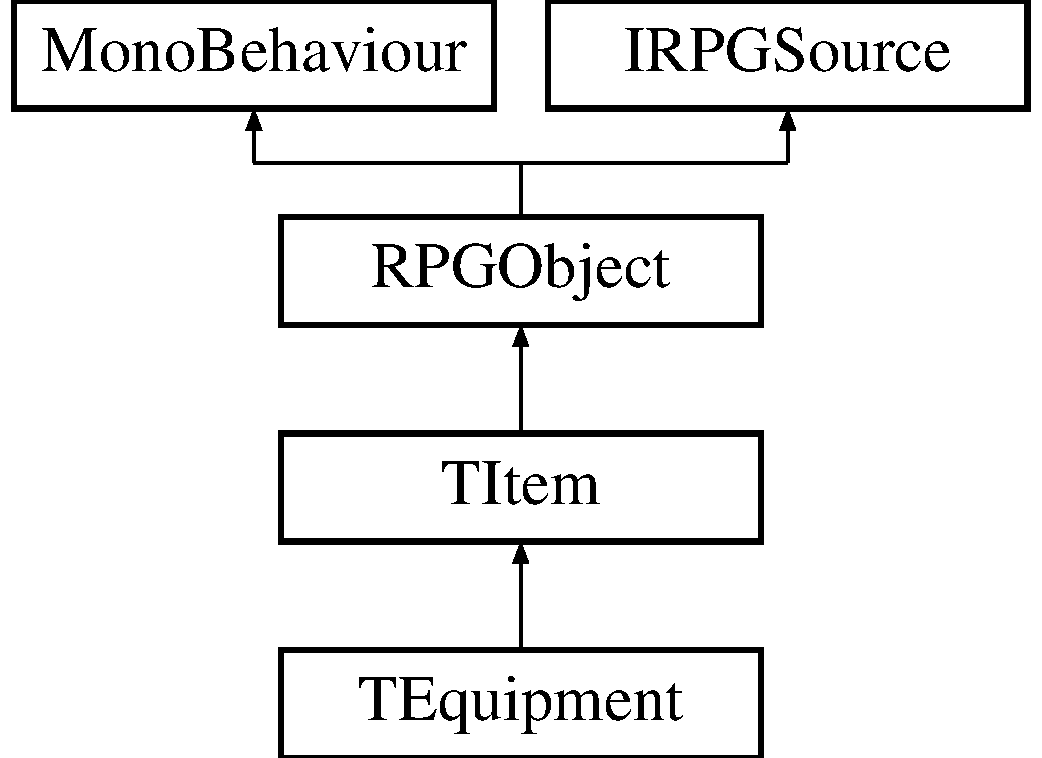
\includegraphics[height=4.000000cm]{class_t_item}
\end{center}
\end{figure}
\subsection*{Public Member Functions}
\begin{DoxyCompactItemize}
\item 
\hypertarget{class_t_item_ae76729202f7144486114a93b9e9dd939}{}override bool {\bfseries Is\+Visible} (out int Hide\+Value, out \hyperlink{class_t_effect}{T\+Effect}\mbox{[}$\,$\mbox{]} Use\+Effects)\label{class_t_item_ae76729202f7144486114a93b9e9dd939}

\item 
\hypertarget{class_t_item_a36fbd6661d50dc4a3e5769b25d59c11e}{}override bool {\bfseries Check\+Value} (string Name\+Of\+Value, out int Base\+Value, out int End\+Value, out \hyperlink{class_t_effect}{T\+Effect}\mbox{[}$\,$\mbox{]} Use\+Effects)\label{class_t_item_a36fbd6661d50dc4a3e5769b25d59c11e}

\item 
\hypertarget{class_t_item_a72a080788b4d4c31b76bea44fef6cd08}{}override float {\bfseries Recieve\+Damage} (float Value, string Typ)\label{class_t_item_a72a080788b4d4c31b76bea44fef6cd08}

\end{DoxyCompactItemize}
\subsection*{Public Attributes}
\begin{DoxyCompactItemize}
\item 
\hypertarget{class_t_item_a2f0849825d38e3b77ccad769a95244d0}{}\hyperlink{class_t_item_statistic}{T\+Item\+Statistic} {\bfseries Original\+Item\+Stats}\label{class_t_item_a2f0849825d38e3b77ccad769a95244d0}

\end{DoxyCompactItemize}
\subsection*{Additional Inherited Members}


The documentation for this class was generated from the following file\+:\begin{DoxyCompactItemize}
\item 
C\+:/\+Users/\+Jordan Eichner/\+Documents/\+Git\+Hub/\+Top\+Down\+R\+P\+G/\+Top\+Down\+R\+P\+G/\+Assets/\+Standard\+Assets/\+R\+P\+G libary/\+Scripts/\+Items/T\+Item.\+cs\end{DoxyCompactItemize}

\hypertarget{class_t_item_statistic}{}\section{T\+Item\+Statistic Class Reference}
\label{class_t_item_statistic}\index{T\+Item\+Statistic@{T\+Item\+Statistic}}


The documentation for this class was generated from the following file\+:\begin{DoxyCompactItemize}
\item 
C\+:/\+Users/\+Jordan Eichner/\+Documents/\+Unity/\+Top\+Down\+R\+P\+G/\+Assets/\+Standard\+Assets/\+R\+P\+G-\/\+Sources/\+Scripts/\+Items/T\+Item\+Statistic.\+cs\end{DoxyCompactItemize}

\hypertarget{class_r_p_g_object_1_1_value_helper}{}\section{R\+P\+G\+Object.\+Value\+Helper Class Reference}
\label{class_r_p_g_object_1_1_value_helper}\index{R\+P\+G\+Object.\+Value\+Helper@{R\+P\+G\+Object.\+Value\+Helper}}
Inheritance diagram for R\+P\+G\+Object.\+Value\+Helper\+:\begin{figure}[H]
\begin{center}
\leavevmode
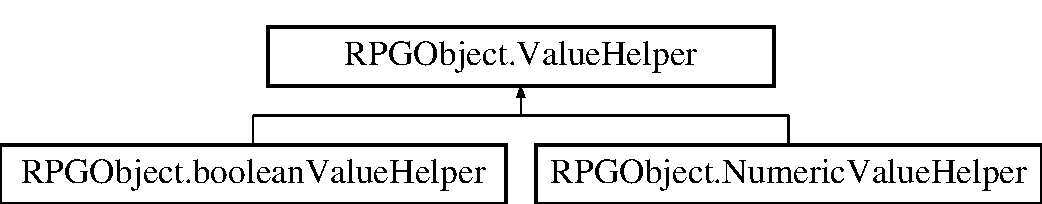
\includegraphics[height=2.000000cm]{class_r_p_g_object_1_1_value_helper}
\end{center}
\end{figure}
\subsection*{Public Attributes}
\begin{DoxyCompactItemize}
\item 
string \hyperlink{class_r_p_g_object_1_1_value_helper_a7e533defe95f542b339bc1a8accab645}{Value\+Name}
\end{DoxyCompactItemize}


\subsection{Detailed Description}
Hilfsklasse um Standardwerte zu verwalten 

\subsection{Member Data Documentation}
\hypertarget{class_r_p_g_object_1_1_value_helper_a7e533defe95f542b339bc1a8accab645}{}\index{R\+P\+G\+Object\+::\+Value\+Helper@{R\+P\+G\+Object\+::\+Value\+Helper}!Value\+Name@{Value\+Name}}
\index{Value\+Name@{Value\+Name}!R\+P\+G\+Object\+::\+Value\+Helper@{R\+P\+G\+Object\+::\+Value\+Helper}}
\subsubsection[{Value\+Name}]{\setlength{\rightskip}{0pt plus 5cm}string R\+P\+G\+Object.\+Value\+Helper.\+Value\+Name}\label{class_r_p_g_object_1_1_value_helper_a7e533defe95f542b339bc1a8accab645}
Name des Werts 

The documentation for this class was generated from the following file\+:\begin{DoxyCompactItemize}
\item 
C\+:/\+Users/\+Jordan Eichner/\+Documents/\+Git\+Hub/\+Top\+Down\+R\+P\+G/\+Top\+Down\+R\+P\+G/\+Assets/\+Standard\+Assets/\+R\+P\+G libary/\+Scripts/\+Meta/R\+P\+G\+Object.\+cs\end{DoxyCompactItemize}

%--- End generated contents ---

% Index
\backmatter
\newpage
\phantomsection
\clearemptydoublepage
\addcontentsline{toc}{chapter}{Index}
\printindex

\end{document}
